\subsection[Scenariusz - man in the middle (Michał Krakowiak)]{Scenariusz - man in the middle}
\subsubsection[Aktorzy]{Aktorzy}
\begin{itemize}
    \item Tester – osoba przeprowadzająca test bezpieczeństwa systemu komputerowego za pomocą dedykowanego systemu
    \item Serwer sterujący – centralny punkt infrastruktury, rejestruje podpięte do sieci Raspberry Pi Zero, przyjmuje polecenia od testera, przekazuje polecenia do Raspberry Pi Zero
    \item Raspberry Pi Zero – niewielkie urządzenie podłączone za pomocą portu USB do testowanego systemu
    \item Testowany system 
\end{itemize}
\subsubsection[Przebieg]{Przebieg}
Test bezpieczeństwa systemu komputerowego za pomocą dedykowanego systemu rozpoczyna się od dostarczenia i instalacji skonfigurowanego Raspberry Pi Zero. Uruchomiona stacja robocza powinna dostarczyć zasilania urządzeniu po przez port USB. Następnie uruchomiony zostaje standardowy element systemu testującego bezpieczeństwo odpowiedzialny za komunikację z serwerem sterującym. Urządzenie rejestruje swoją obecność i jest gotowe do przyjmowania poleceń wydawanych przez serwer.
Resztę działań tester przeprowadza zdalnie. Z poziomu przeglądarki, po zalogowaniu do aplikacji, może wskazać jedno lub więcej urządzeń zarejestrowanych w systemie. Następnie uruchamiany jest kreator testu bezpieczeństwa, który pozwala testerowi zlecić zebranie ruchu sieciowego generowanego przez stacje robocze. Tester ponadto ma możliwość ustawienia takich parametrów jak czas trwania operacji oraz częstotliwości raportowania danych do serwera sterującego.
Po poprawnym przyjęciu żądanej operacji serwer sterujący przekazuje ją do wskazanych urządzeń. Raspberry Pi Zero identyfikuje polecenie przechwycenia ruchu sieciowego i rozpoczyna wykonywanie skryptów inicjujących wskazanych funkcjonalności. Raspberry Pi Zero rejestruje swoją obecność w testowanym systemie komputerowym jako zewnętrzna karta sieci Ethernet. Następnie rozsyłane są odpowiednio spreparowane ustawienia DHCP dla nowo przyłączonego interfejsu ethernetowego w testowanym systemie. Mają one zapewnić, że ruch sieciowy zostanie przekierowany do Raspberry Pi Zero. Użytkownik systemu komputerowego generuje ruch sieciowy po przez m.in. korzystanie z przeglądarki, który jest przekazywany do podłączonego w sposób transparentny. Przechodzące dane są zapisywane w pamięci wewnętrznej urządzenia. Po upłynięciu ustalonego przez testera czasu zebrane informacje zostają przesłane do serwera sterującego w celu umożliwienia ich późniejszej analizy.
\begin{figure}[H]
    \centering
    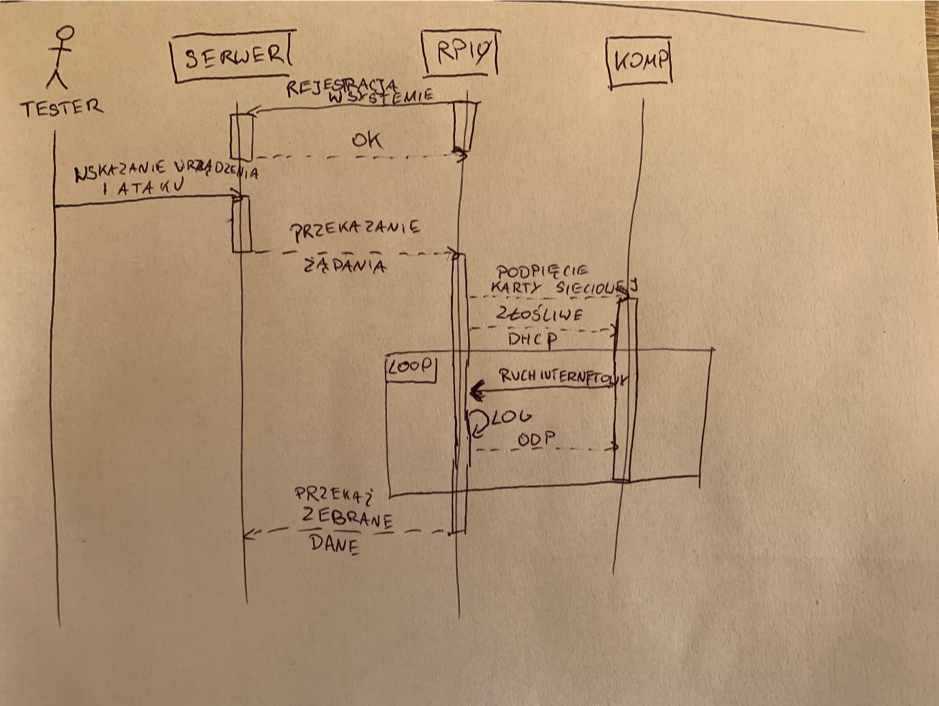
\includegraphics[width=\textwidth]{mk05}
    \caption{Mitm}
    \label{fig:mitm}    
\end{figure}